\documentclass[conference]{IEEEtran}

\usepackage{graphicx}
\usepackage{amsmath}
\usepackage{url}
\usepackage{float}
\usepackage{cite}
\usepackage{array}
\usepackage{booktabs}
\usepackage{titlesec}
\usepackage{hyperref}

% ---------- Section Spacing ----------
\titlespacing*{\section}
{0pt}{1.2ex plus .2ex minus .2ex}{0.8ex}

\titlespacing*{\subsection}
{0pt}{0.8ex plus .2ex minus .2ex}{0.5ex}

\titlespacing*{\subsubsection}
{0pt}{0.6ex plus .2ex minus .2ex}{0.4ex}

% ---------- Paragraph Spacing ----------
\setlength{\parskip}{0pt}
\setlength{\parindent}{1em}

% ---------- Figure/Table Spacing ----------
\setlength{\textfloatsep}{8pt}
\setlength{\floatsep}{8pt}
\setlength{\intextsep}{8pt}

% ---------- List Spacing ----------
\usepackage{enumitem}
\setlist[itemize]{noitemsep, topsep=2pt}
\setlist[enumerate]{noitemsep, topsep=2pt}

\title{Anti-Theft Smart Locker System Using ESP32}

\author{
\IEEEauthorblockN{Dipanshu, Atul Kumar, Kunal, Rahul Yadav}
\IEEEauthorblockA{
Department of Computer Science and Engineering\\
Lovely Professional University, Punjab, India\\
Guide: Neha Kapila
}
}

\begin{document}

\maketitle
\textbf{Group Member Details}

\vspace{0.15cm}

\renewcommand{\arraystretch}{1.2}

\resizebox{1.0\columnwidth}{!}{
\begin{tabular}{|c|c|c|c|}
\hline
\textbf{Name} & \textbf{Roll No.} & \textbf{Section} & \textbf{Registration No.} \\
\hline
Dipanshu & 39 & 225UK & 12508828 \\
\hline
Atul Kumar & 50 & 225UK & 12505051 \\
\hline
Kunal & 64 & 225UK & 12508893 \\
\hline
Rahul Yadav & 44 & 225UK & 12506486 \\
\hline
\end{tabular}
}

\vspace{0.75cm}

% ================= ABSTRACT =================
\begin{abstract}
The proposed system provides reliable intrusion detection, real-time alerting, and automated asset protection through an intelligent hidden-compartment mechanism.
\end{abstract}

\begin{IEEEkeywords}
ESP32, Embedded System, IoT, Smart Locker, Security System
\end{IEEEkeywords}

% ================= I =================
\section{INTRODUCTION}

In contemporary living, security of personal property is of the utmost importance. Many individuals keep jewelry, money, documents and electronic devices in lockers; assuming complete security. Current locker models only have basic mechanisms for locking and do not provide real-time monitoring of the use of the locker.

With the rapid advancement of Internet of Things (IoT) and embedded technologies, traditional security systems can be transformed into intelligent and automated protection systems. Smart lockers can authenticate users, detect intrusion attempts, trigger alarms, and transmit real-time notifications through internet-based communication.

In this project, an \textbf{ESP32} will be utilized as a central controller which will handle the authentication process, detect theft attempts and trigger alarms for a single user. The \textbf{ESP32 microcontroller} is ideal for these applications due to its integrated Wi-Fi capability, processing speed and multiple sensor interfaces.

A \textbf{microcontroller} is a compact programmable integrated circuit used to control electronic systems.  
An \textbf{embedded system} is a dedicated computing system designed for a specific function.

Security is a major concern in modern environments. Traditional lockers lack intelligent monitoring and fail to provide real-time alerts. This project introduces a smart locker system using \textbf{ESP32}that integrates authentication, sensing, and communication technologies.

The system detects unauthorized access and secures valuables using a hidden compartment, making it more advanced than conventional lockers.

% ================= II =================
\section{LITERATURE REVIEW}

\begin{enumerate}

\item \textbf{Sudha Kousalya, G. Reddi Priya, R. Vasanthi, and B. Venkatesh (2018)} presented an IoT-based smart security and home automation system using Arduino and sensors. Their system focused on real-time monitoring, remote control, and automation using internet communication. The research demonstrated how embedded systems can improve security and convenience in modern environments. Their work also emphasized the importance of low-cost IoT-based smart security solutions.

\item \textbf{Mohamed Faisal Elrawy, Ali Ismail Awad, and Hesham F. A. Hamed (2018)} discussed intrusion detection systems for IoT-based smart environments. Their study highlighted threats such as unauthorized access, malware attacks, and insecure communication in connected systems. The researchers proposed secure authentication and communication mechanisms to improve IoT security and reliability.

\item \textbf{Muhammad Burhan, Rana Asif Rehman, Bilal Khan, and Byung-Seo Kim (2018)} proposed layered IoT architectures and analyzed vulnerabilities in cloud-connected embedded devices. Their research focused on scalability, secure communication, and interoperability in IoT systems. The study emphasized the need for strong protection mechanisms in smart connected environments.

\item \textbf{Kejun Chen, Shuai Zhang, Zhikun Li, and Yier Jin (2018)} investigated security threats and vulnerabilities in Internet of Things applications. Their study discussed malware attacks, privacy issues, and unauthorized access in smart systems. The researchers also proposed security countermeasures to improve data protection and system reliability.

\item \textbf{Aditya Kumar, Shipra Saraswat, and Saurabh Singh (2018)} developed a laser-based IoT security system using Arduino and infrared sensors. Their system detected intrusion attempts and generated real-time alerts using internet communication. The project demonstrated an affordable and efficient embedded security solution for smart environments.

\item \textbf{T. Pavan Kumar, R. Hemanth Krishna, M. Sai Krishna, and Jhanavi Meghana (2018)} implemented a smart home automation system integrated with IoT communication and sensor monitoring. Their research focused on remote control, automation, and security enhancement using embedded technologies. The study showed the effectiveness of IoT in intelligent monitoring systems.

\item \textbf{Deepti Sehrawat and Nasib Singh Gill (2018)} analyzed major challenges in IoT deployment including scalability, privacy, security, and communication reliability. Their work highlighted the importance of secure data transfer and efficient network management in smart environments. The study provided insights into limitations and future improvements in IoT systems.

\item \textbf{Imran Makhdoom, Mehran Abolhasan, Justin Lipman, and Ren Ping Liu (2018)} explored cyber threats and security challenges in IoT systems. Their research discussed secure communication methods, encryption techniques, and authentication systems for protecting smart devices. The study emphasized the importance of cybersecurity in embedded and IoT applications.

\item \textbf{Amit Kumar Sikder, Giuseppe Petracca, Hidayet Aksu, Trent Jaeger, and A. Selcuk Uluagac (2018)} surveyed sensor-based attacks in IoT systems and discussed vulnerabilities associated with embedded sensors. Their work proposed security mechanisms to improve sensor reliability and prevent unauthorized access in smart devices.

\item \textbf{Vishal Sharma, Ilsun You, Karl Andersson, and Francesco Palmieri (2019)} studied trust management, privacy protection, and secure communication techniques for IoT-based mobile systems. Their research focused on authentication methods, secure data exchange, and cloud-connected applications. The study contributed toward improving reliability and security in IoT communication networks.

\end{enumerate}

% ================= III =================
\section{PROBLEM STATEMENT}

Traditional locker systems suffer from several limitations:

\begin{itemize}
    \item No real-time monitoring or alert mechanism
    \item Keys can be lost, duplicated, or easily compromised
    \item No intrusion detection for unauthorized access attempts
    \item No remote notification system for the owner
    \item Delayed response during theft or tampering incidents
    \item No fallback system on breach
\end{itemize}

Therefore, an intelligent security solution is required that can automatically detect suspicious activity, notify the user in real time, and protect valuables more effectively.

% ================= IV =================
\section{OBJECTIVES}

\begin{itemize}
    \item To design a smart locker system using ESP32
    \item To implement password-based authentication
    \item To detect unauthorized access using a vibration sensor
    \item To generate real-time theft alerts through IoT communication
    \item To activate a hidden safety compartment during intrusion attempts
    \item To develop a web-based monitoring dashboard
    \item To enhance security compared to conventional lockers
\end{itemize}

% ================= V =================
\section{SYSTEM DESIGN}

\subsection{Methodology of Model Development}

\textbf{Methodology} is a structured approach used to design and implement a system.

Steps:
\begin{enumerate}
\item Password input via keypad
\item Validation by ESP32
\item Servo control for locking
\item Vibration detection
\item Alert triggering
\item Telegram and Web notification
\end{enumerate}

\subsection{Hardware Module Design}

The proposed Anti-Theft Smart Locker System consists of multiple hardware modules integrated to provide authentication, intrusion detection, automated locking, and IoT-based monitoring.

The \textbf{ESP32 microcontroller} acts as the central controller of the system. It processes sensor data, validates passwords, controls output devices, and manages Wi-Fi communication.

A \textbf{4x4 keypad} is used for password entry, while a \textbf{servo motor} controls the locking and unlocking mechanism of the locker. The \textbf{SW-420 vibration sensor} detects tampering or forced access attempts and sends signals to the ESP32 for security action.

A \textbf{16x2 LCD display} with an \textbf{I2C module} is used to display system messages and authentication status. A \textbf{buzzer} generates alarm sounds during unauthorized access attempts.

All components are connected using jumper wires to form a compact and intelligent embedded security system.

\subsection{Block Diagram}

A \textbf{block diagram} is a graphical representation of the system components. It is a high-level visual representation of a system, using labeled rectangles (blocks) to represent major components or functions and lines to show their relationships, signal flow, or interactions. Focuses on the general structure and functionality, rather than detailed technical implementation.

\begin{figure}[H]
\centering
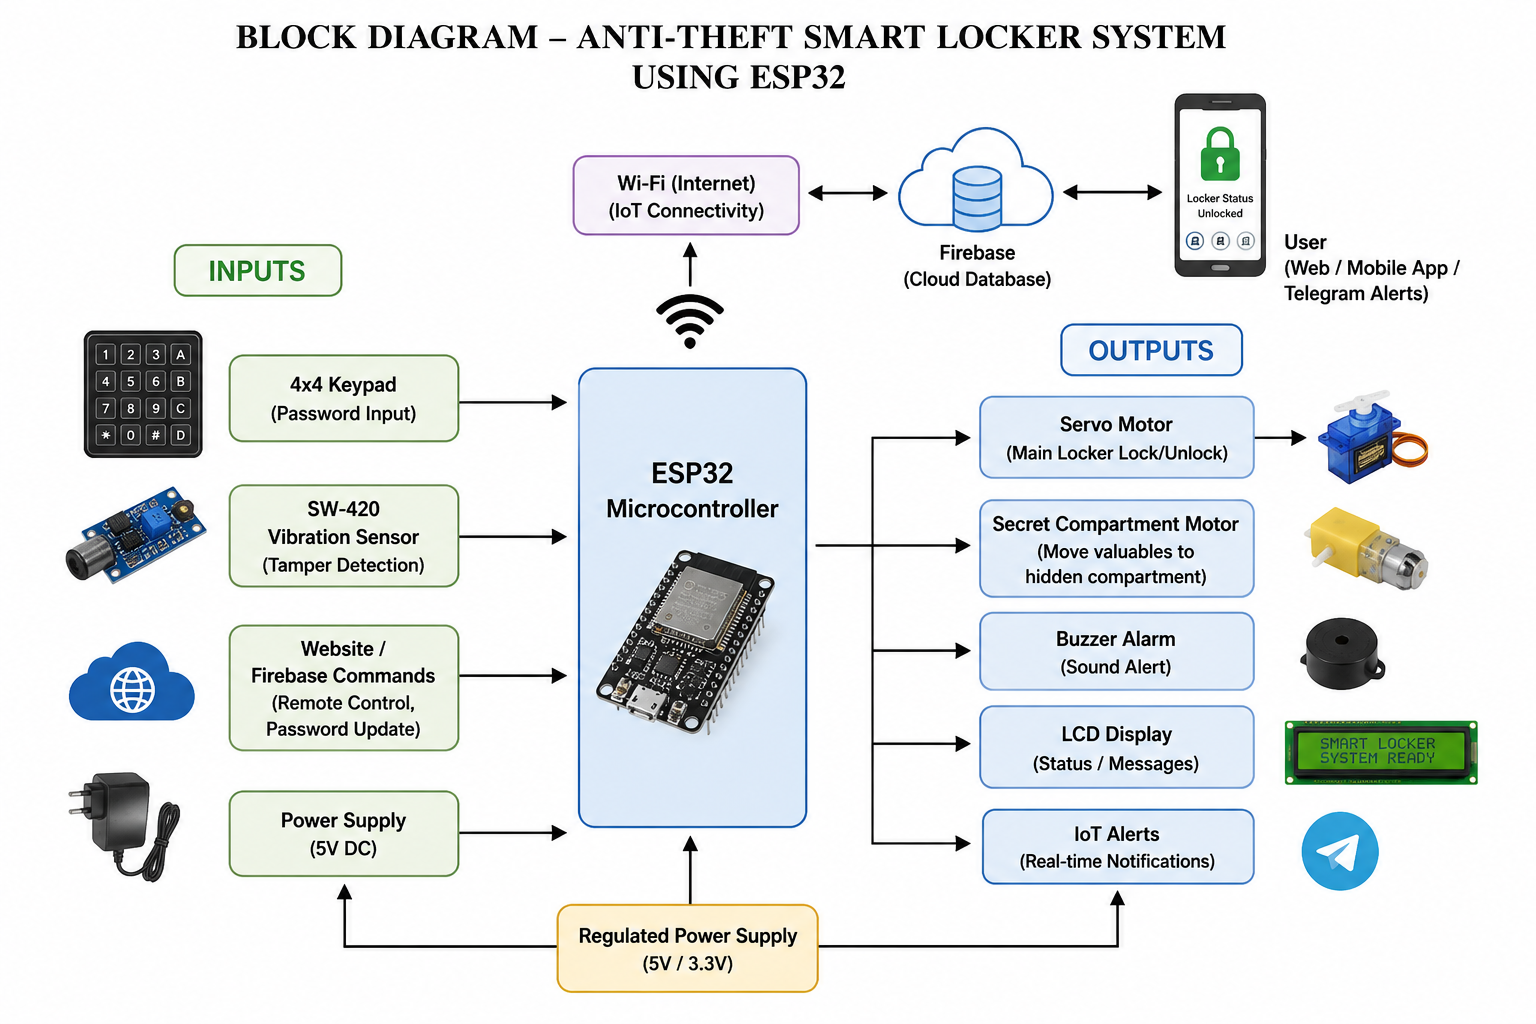
\includegraphics[width=0.45\textwidth]{block-diagram.png}
\caption{Block Diagram}
\end{figure}

\begin{figure}[H]
\centering
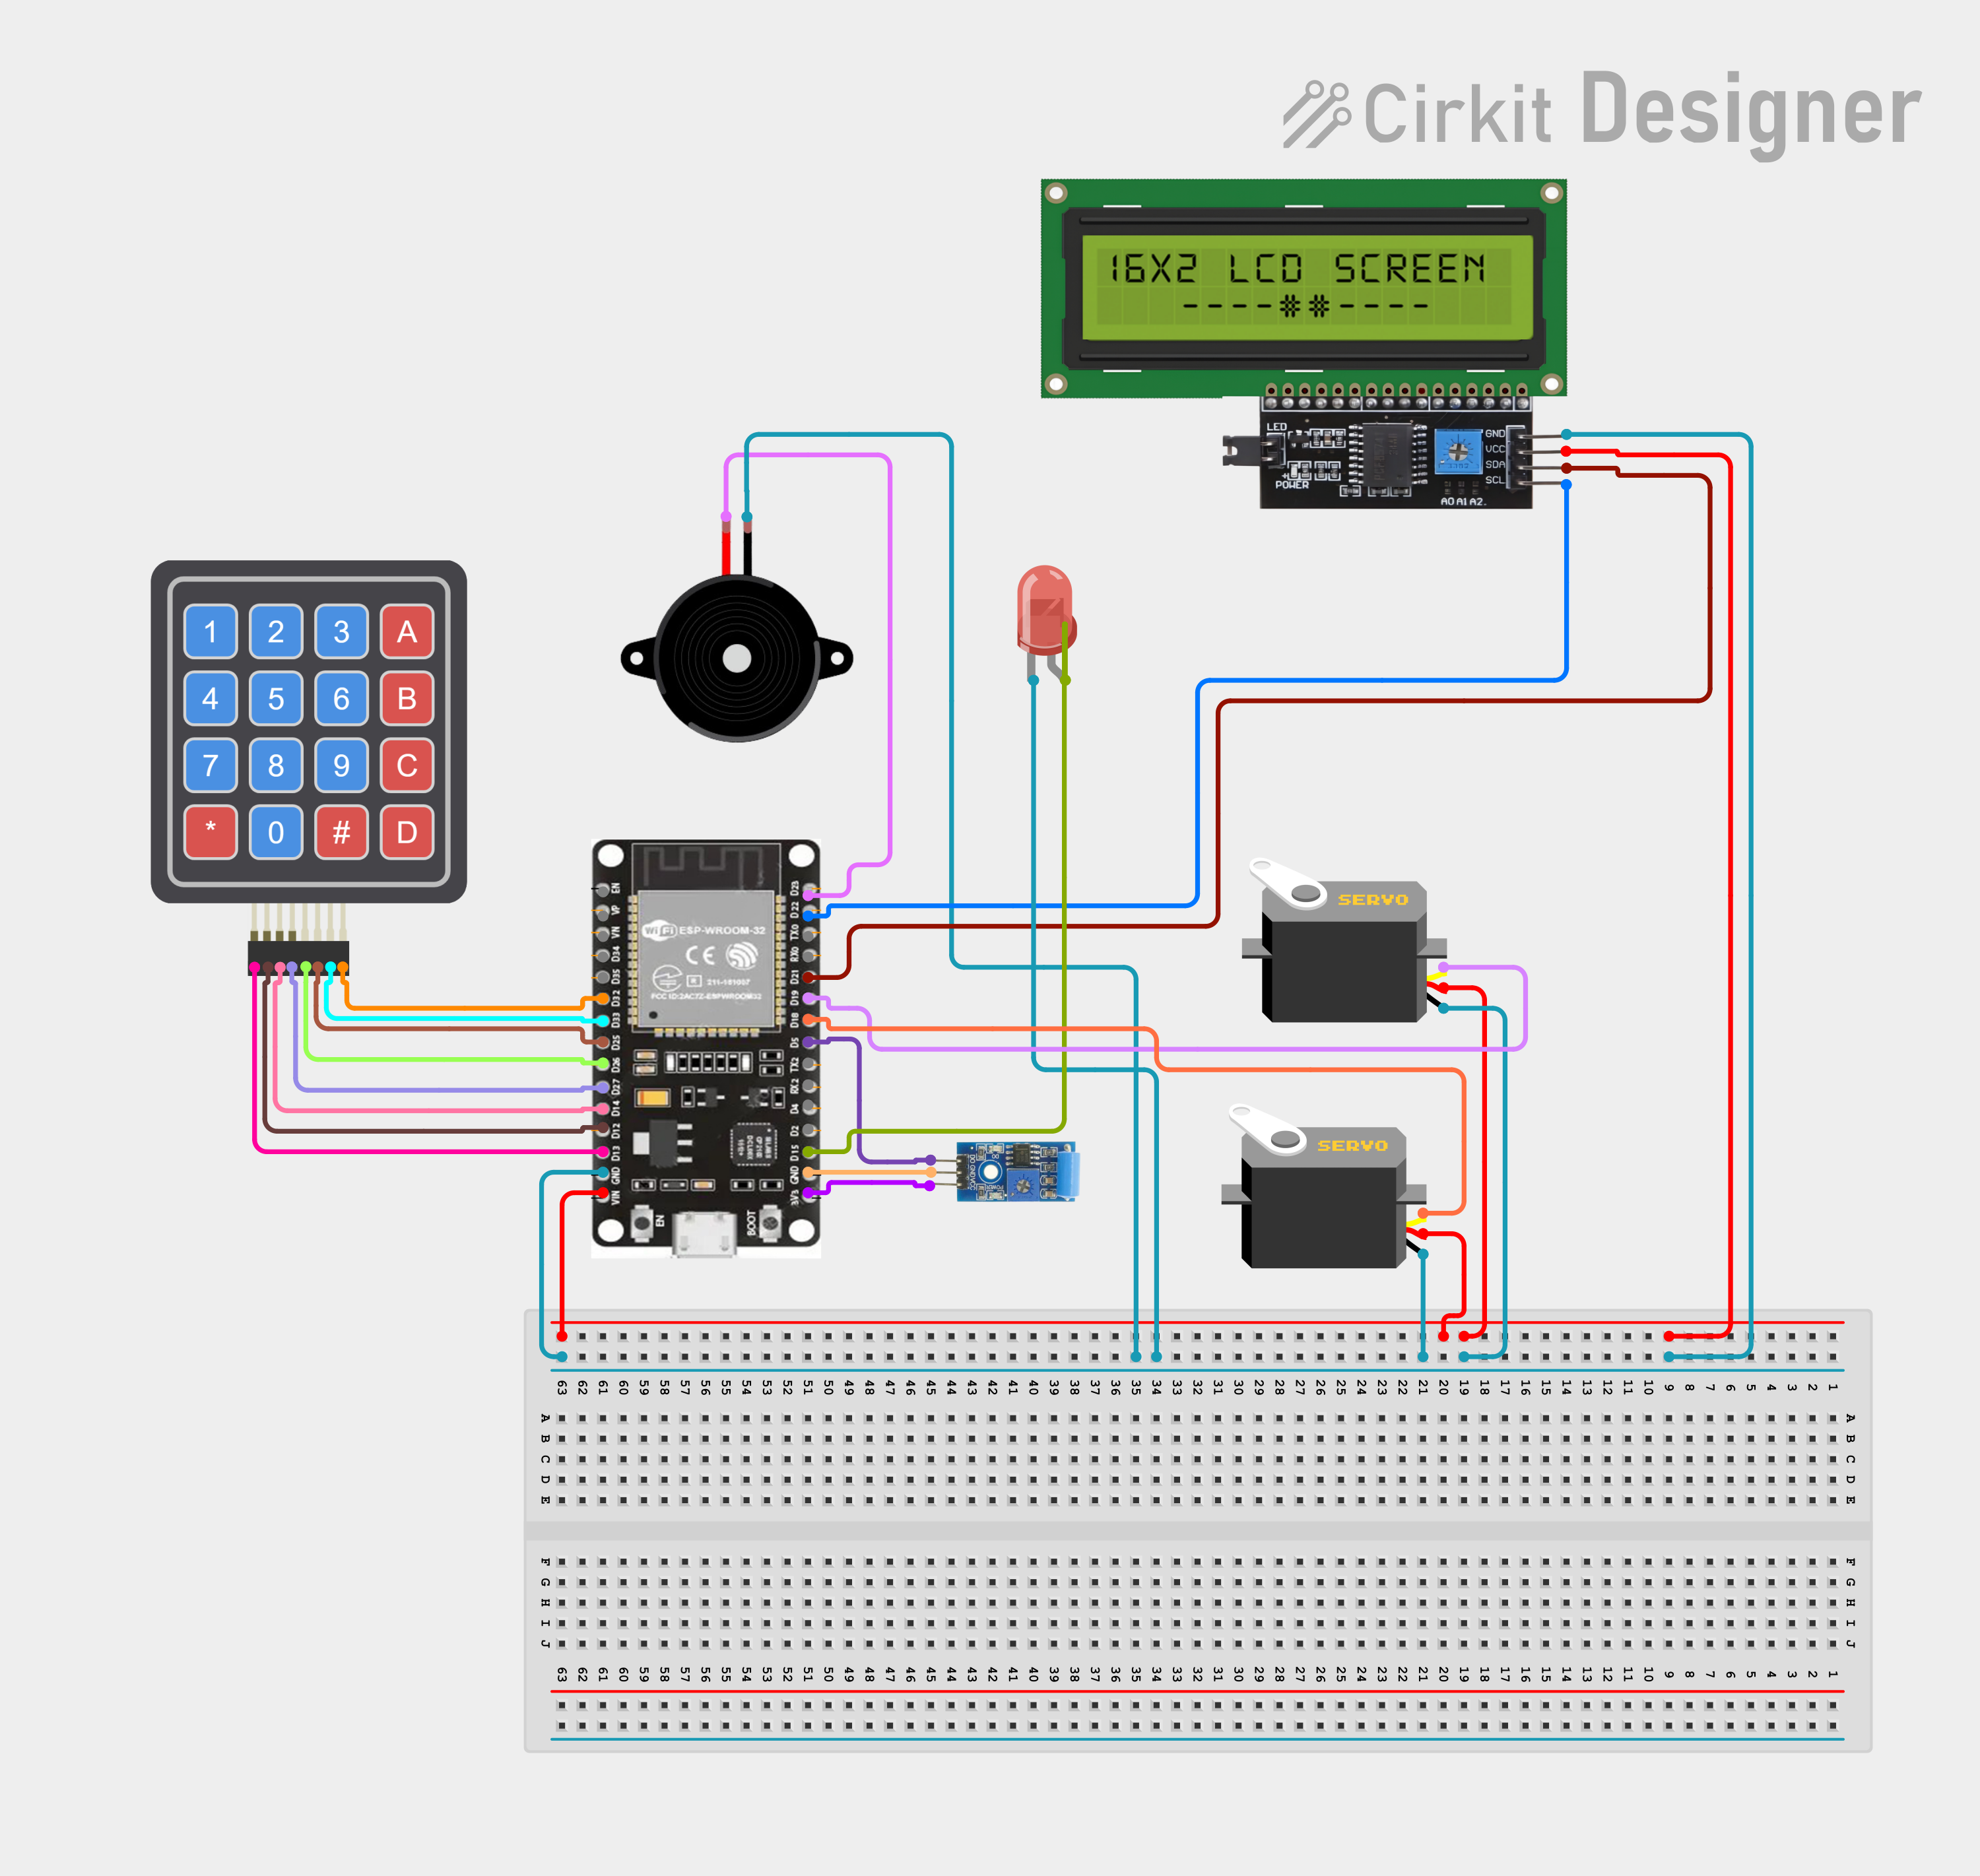
\includegraphics[width=0.45\textwidth]{circuit.png}
\caption{Circuit Diagram of Smart Locker System}
\end{figure}

% ================= VI =================
\section{HARDWARE DESCRIPTION}
\subsection{ESP32}
\textbf{ESP32} is a highly capable microcontroller that integrates Wi-Fi as well as Bluetooth (BLE). This device provide many GPIOs (input/output pins), low power consumption, as well as fast performance and can also be used to control all the sensors attached to an output device within a single system.

\begin{figure}[H]
\centering
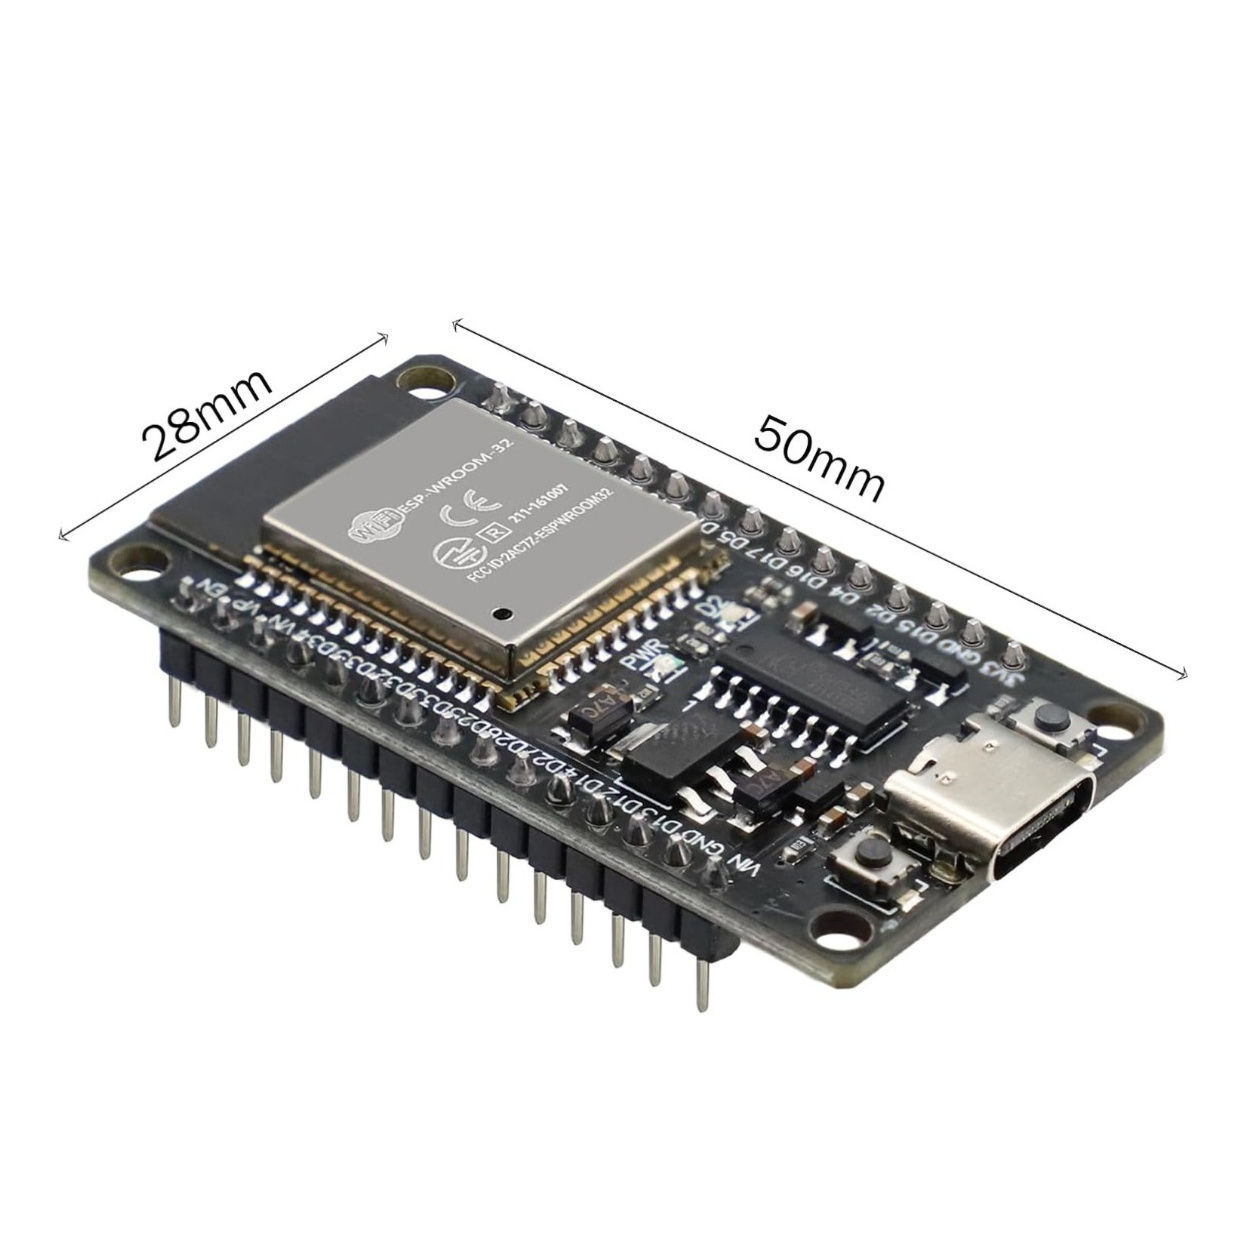
\includegraphics[width=0.3\textwidth]{esp32.jpg}
\caption{ESP32 Module}
\end{figure}

\subsection{Keypad}
A \textbf{keypad} is an input device that is used to enter passwords. It is a peripheral input device utilized in embedded systems to capture alphanumeric user input. It provides a highly efficient method for integrating multiple tactile switches into a circuit while minimizing the hardware resources required from the host microcontroller, such as an Arduino or ESP32.

\begin{figure}[H]
\centering
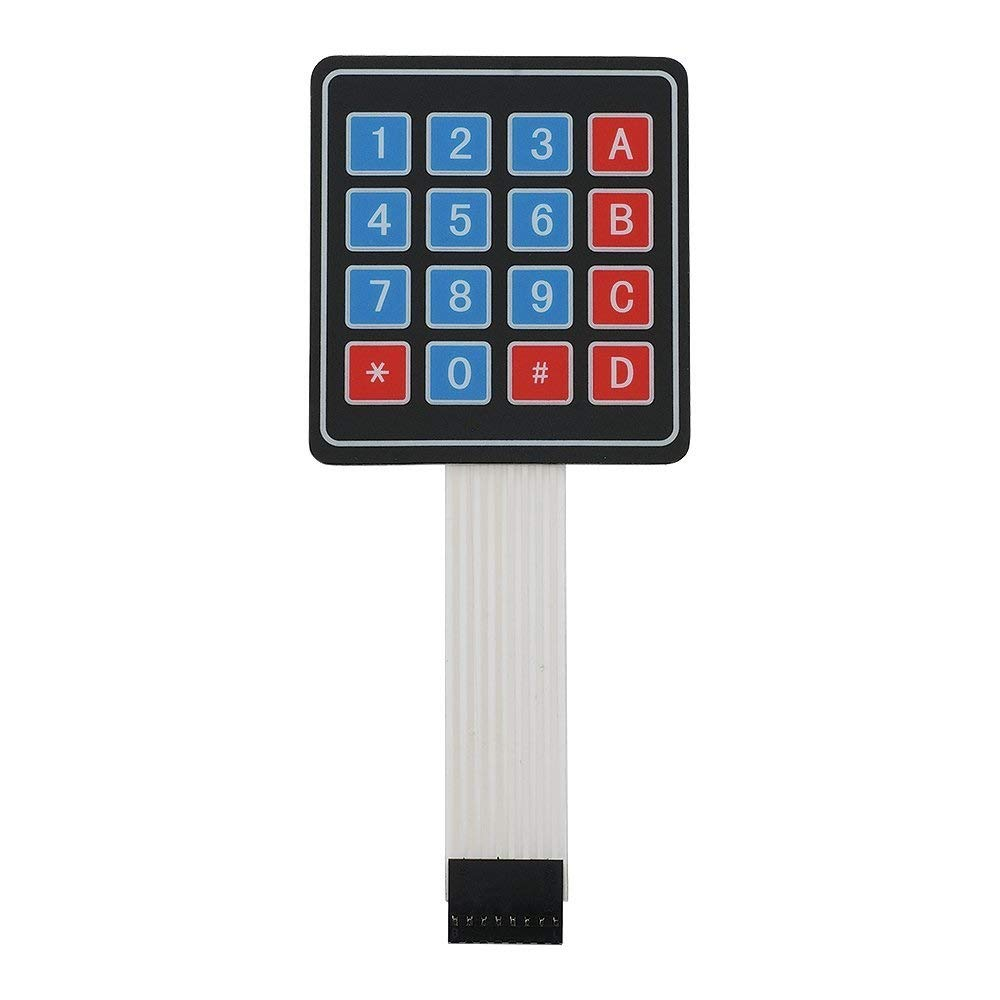
\includegraphics[width=0.3\textwidth]{keypad.jpg}
\caption{4x4 Keypad}
\end{figure}

\subsection{Servo Motor}
The \textbf{Servo Motor} is a high-precision rotary actuator designed for accurate control of angular position, velocity, and acceleration. Unlike standard DC motors that rotate continuously, a servo is engineered for applications where specific positioning is critical.

\begin{figure}[H]
\centering
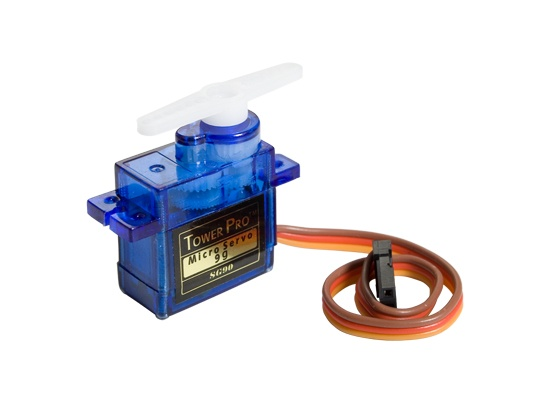
\includegraphics[width=0.3\textwidth]{servo.jpg}
\caption{Servo Motor}
\end{figure}

\subsection{Vibration Sensor}
\textbf{SW-420 Vibration Sensor} is a module that can detect vibrations or shocks on a surface. It can be used for various purposes, such as detecting door knocks, machine malfunctions, car collisions, or alarm systems. It operates from 3.3 V to 5 V. The module has three peripherals, two LEDs, one for the power status and the other for the sensor output. In addition, there is a potentiometer that can be further used to control the threshold point of the vibration.


\begin{figure}[H]
\centering
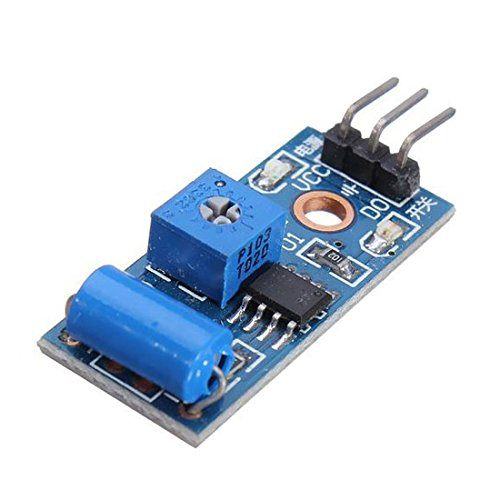
\includegraphics[width=0.3\textwidth]{vibration-sensor.jpg}
\caption{Vibration Sensor (SW-420)}
\end{figure}

\subsection{LCD Display}
A \textbf{16x2 LCD} is a basic, affordable, and widely used Liquid Crystal Display module capable of showing 32 alphanumeric characters across two rows, with 16 characters per row

\begin{figure}[H]
\centering
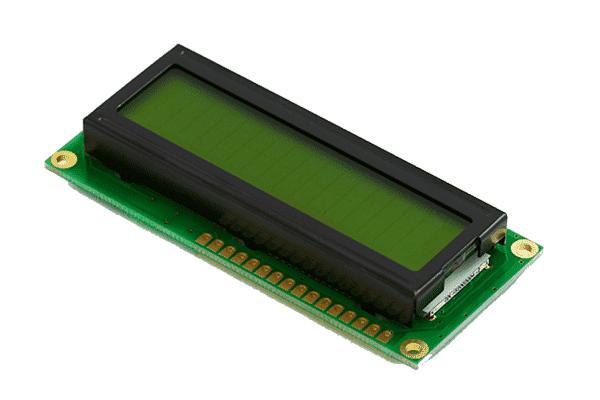
\includegraphics[width=0.3\textwidth]{lcd.png}
\caption{16x2 LCD}
\end{figure}

\subsection{I2C Module}
An \textbf{I2C Module} enables communication with microcontrollers like Arduino or ESP32 using only two data pins (SDA and SCL) instead of the 10+ wires required for parallel mode.

\begin{figure}[H]
\centering
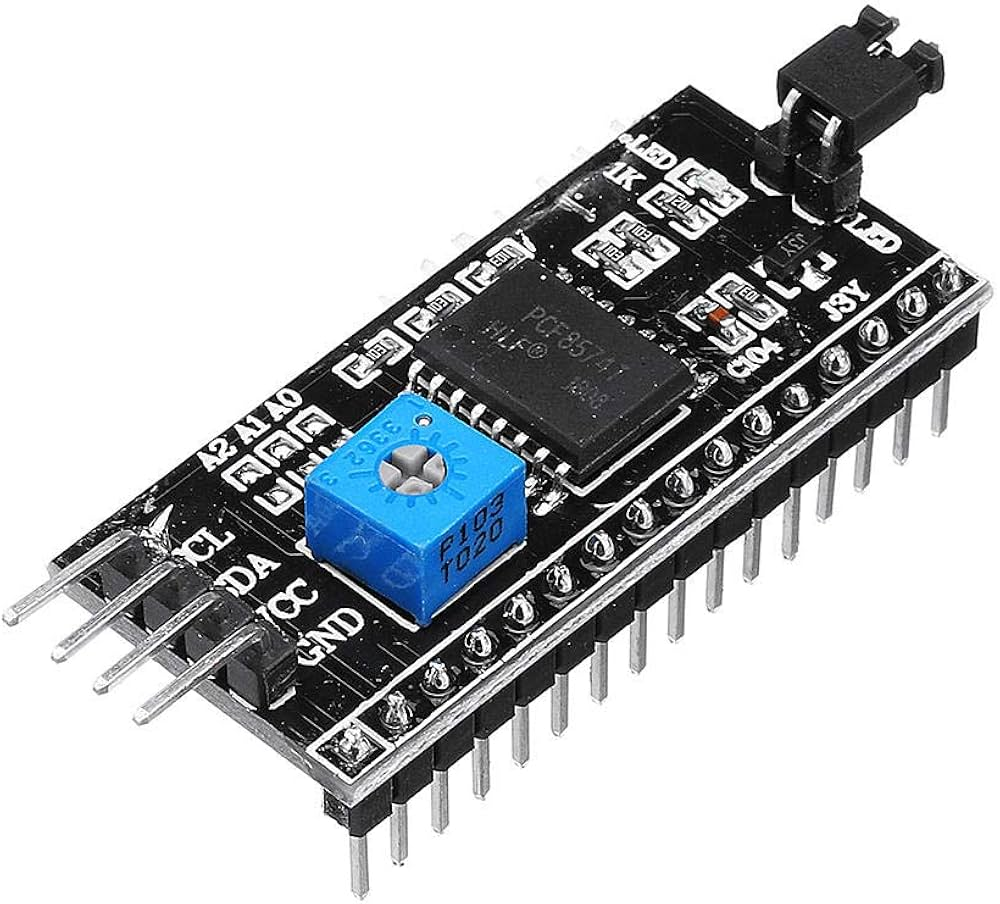
\includegraphics[width=0.3\textwidth]{i2c.jpg}
\caption{I2C Module}
\end{figure}

\subsection{Jumper Wires}
Jumper wires are flexible electrical cables used in
electronics. They have connectors at both ends and are
often made of thin copper wire with insulation. They're
handy for creating temporary connections between
components on breadboards or circuit boards during
testing or prototyping.

\begin{figure}[H]
\centering
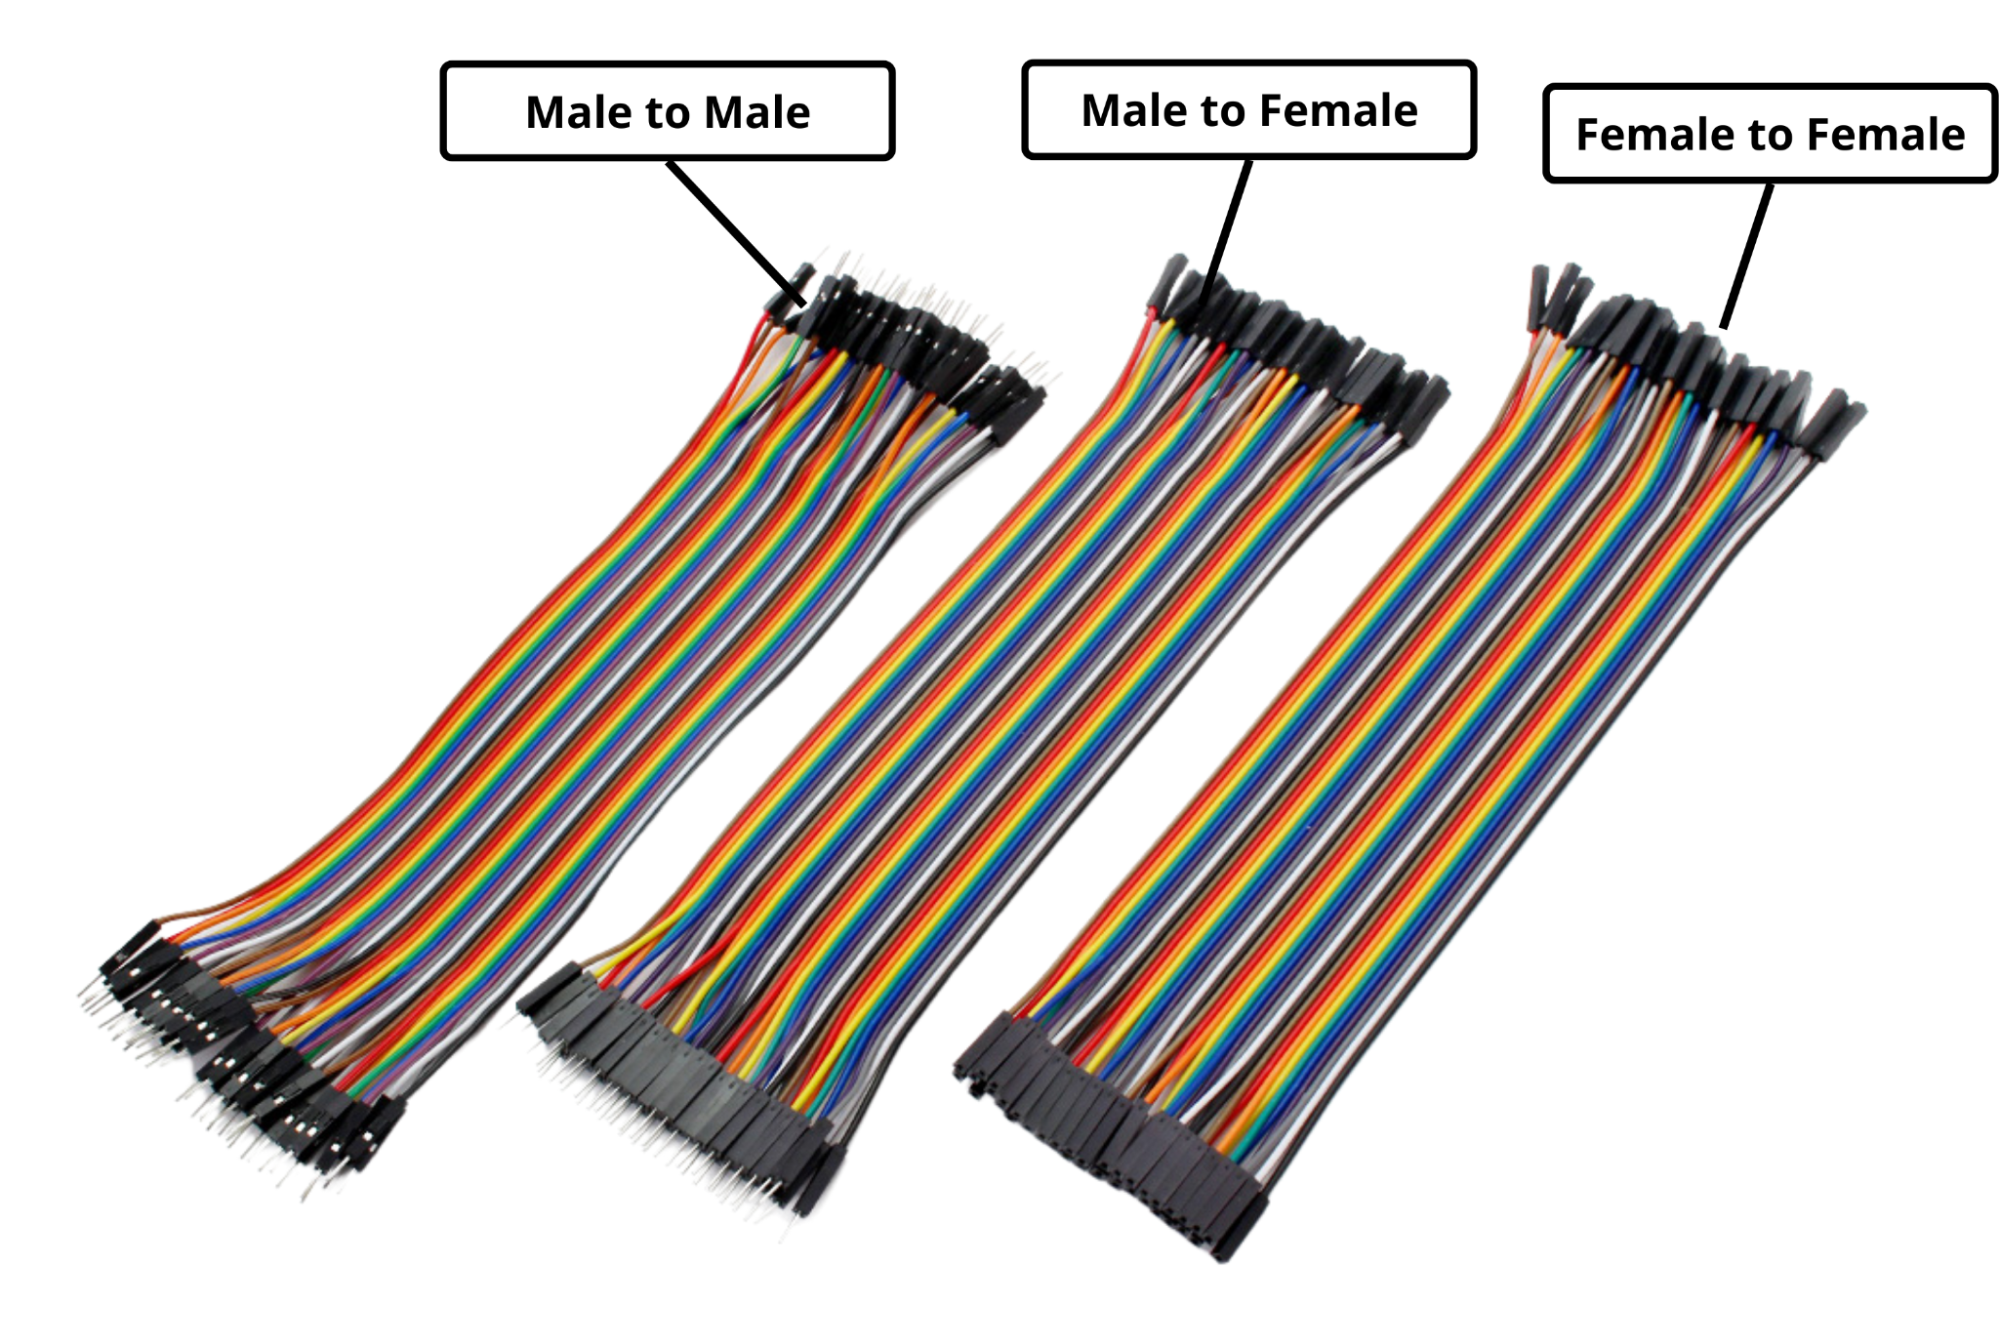
\includegraphics[width=0.3\textwidth]{jumper-wires.png}
\caption{Jumper Wires (M2M, F2F, M2F)}
\end{figure}

% ================= VII =================
\section{HARDWARE WORKING}

The system works by combining input, processing, and output.
When a password is entered, ESP32 validates it. If correct, the servo unlocks the locker. If incorrect, attempts increase and an alert is triggered after 3 failures.
If unauthorized vibration or tampering is detected, the buzzer alarm is activated and the secret compartment mechanism secures the valuables automatically.

% ================= VIII =================
\section{SOFTWARE OVERVIEW}

An \textbf{IDE (Integrated Development Environment)} is software used to develop programs.

The software implementation is developed using Arduino IDE with libraries including Keypad, ESP32Servo, WiFi, HTTPClient, and LiquidCrystal I2C for hardware interfacing and IoT communication.

\begin{figure}[H]
\centering
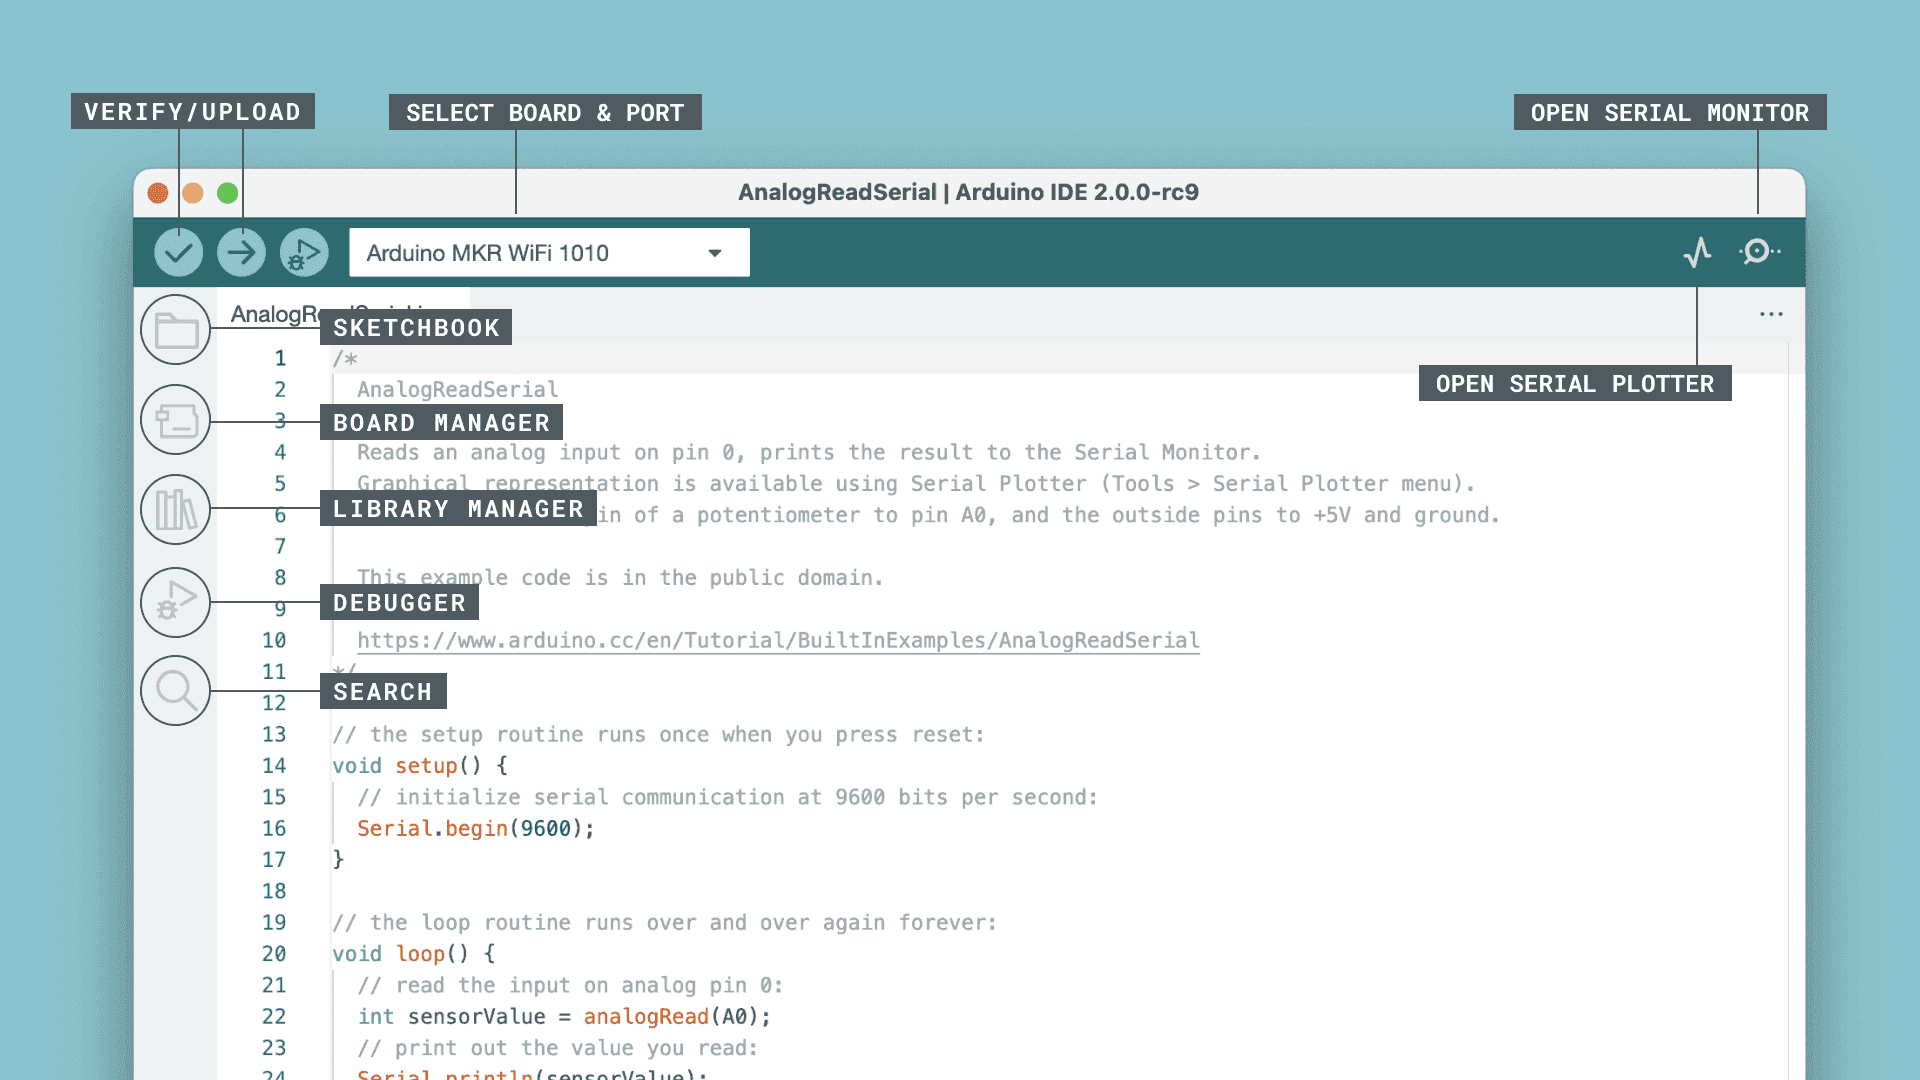
\includegraphics[width=0.45\textwidth]{arduino_ide.png}
\caption{Arduino IDE}
\end{figure}

% ================= IX =================
\section{SOFTWARE IMPLEMENTATION}

The software implementation of the proposed Anti-Theft Smart Locker System is developed using the \textbf{ESP32 microcontroller}, \textbf{Firebase Realtime Database}, and a \textbf{React-based web application}. The software controls authentication, intrusion detection, IoT communication, cloud synchronization, and real-time monitoring.

The ESP32 acts as the central processing unit of the system. It continuously reads sensor inputs, validates password data, controls actuators, and exchanges real-time information with the cloud database through Wi-Fi communication.

\begin{figure}[H]
\centering
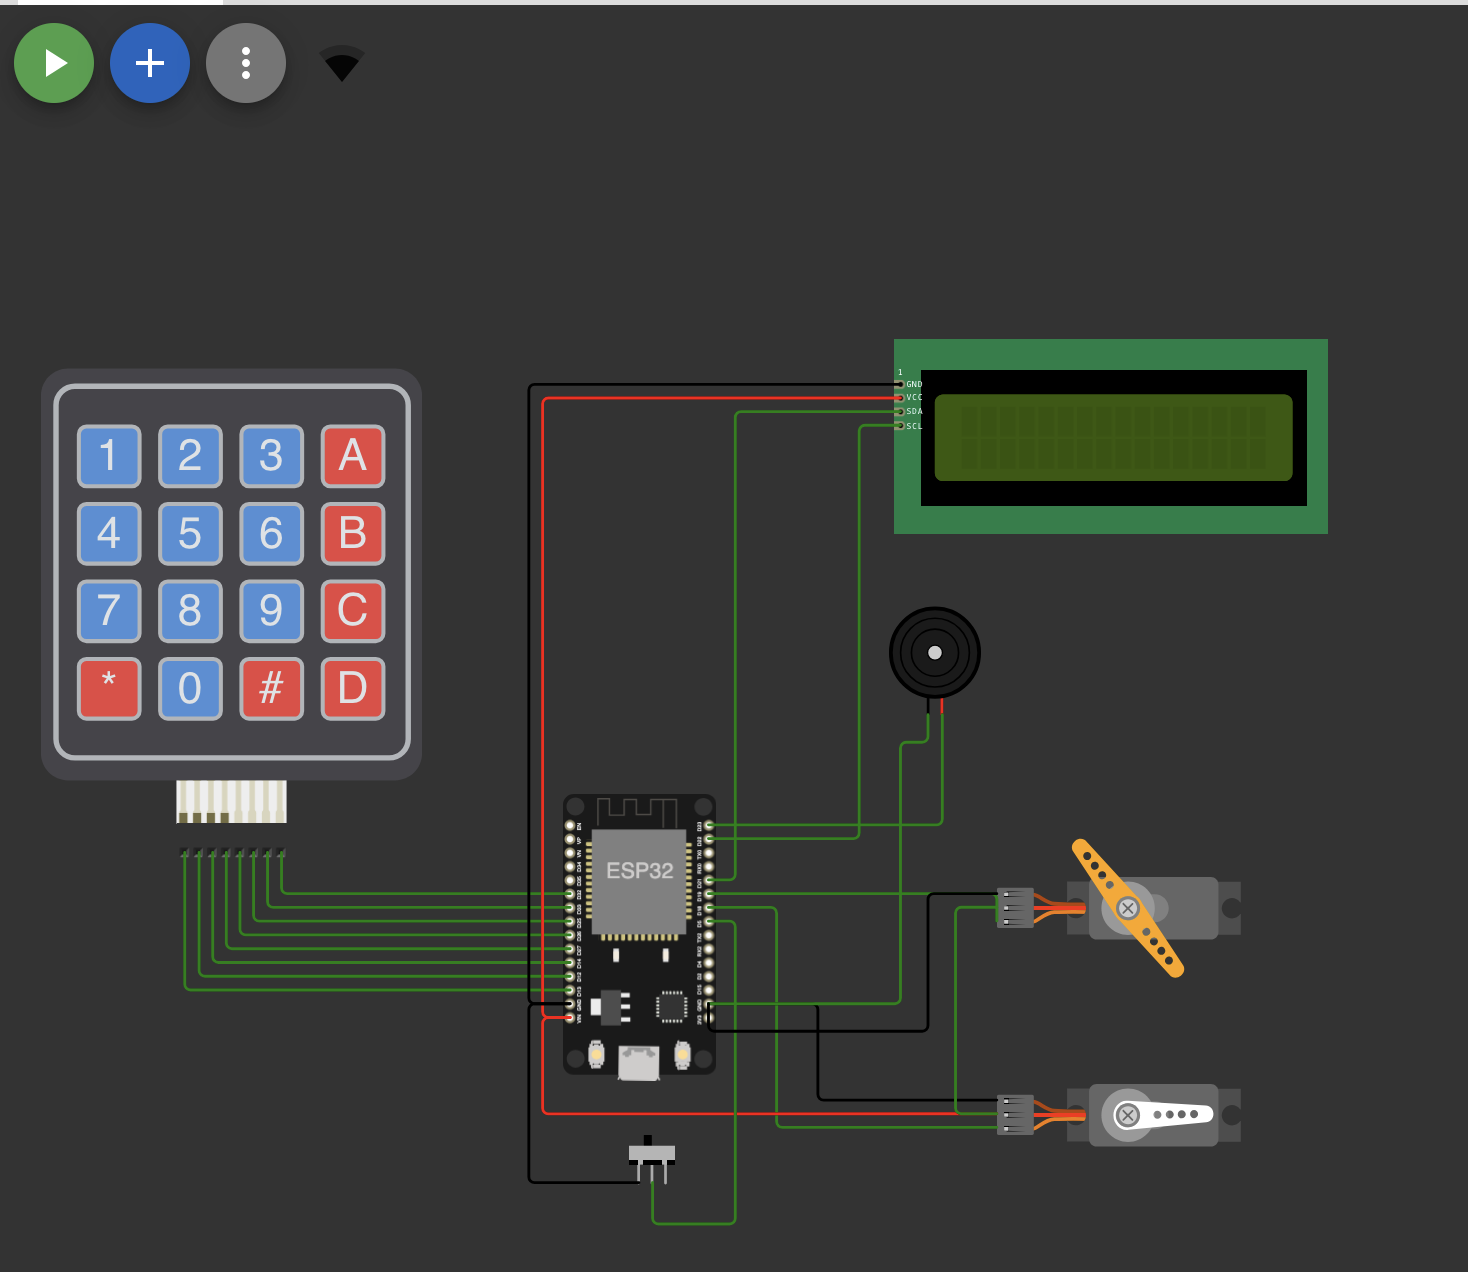
\includegraphics[width=0.45\textwidth]{wokwi-simulation.png}
\caption{Simulation of Smart Locker System}
\end{figure}

\subsection{System Workflow}

The complete software workflow operates as follows:

\begin{enumerate}

\item The system initializes all peripherals including the keypad, LCD display, servo motor, vibration sensor, buzzer, and Wi-Fi module.

\item The user enters the password using the 4×4 matrix keypad.

\item The ESP32 compares the entered password with the stored password data.

\item If the password is correct:
\begin{itemize}
\item The servo motor unlocks the locker.
\item Access is granted to the user.
\item The LCD displays a success message.
\item System status is updated on the web dashboard.
\end{itemize}

\item If the password is incorrect:
\begin{itemize}
\item The attempt counter increases.
\item Warning messages are displayed on the LCD.
\item Unauthorized activity is logged in the cloud database.
\end{itemize}

\item After three incorrect attempts:
\begin{itemize}
\item The buzzer alarm is activated.
\item The secret compartment mechanism is triggered.
\item Real-time theft alerts are sent through Telegram/web dashboard notifications.
\item The system enters theft protection mode.
\end{itemize}

\begin{figure}[H]
\centering
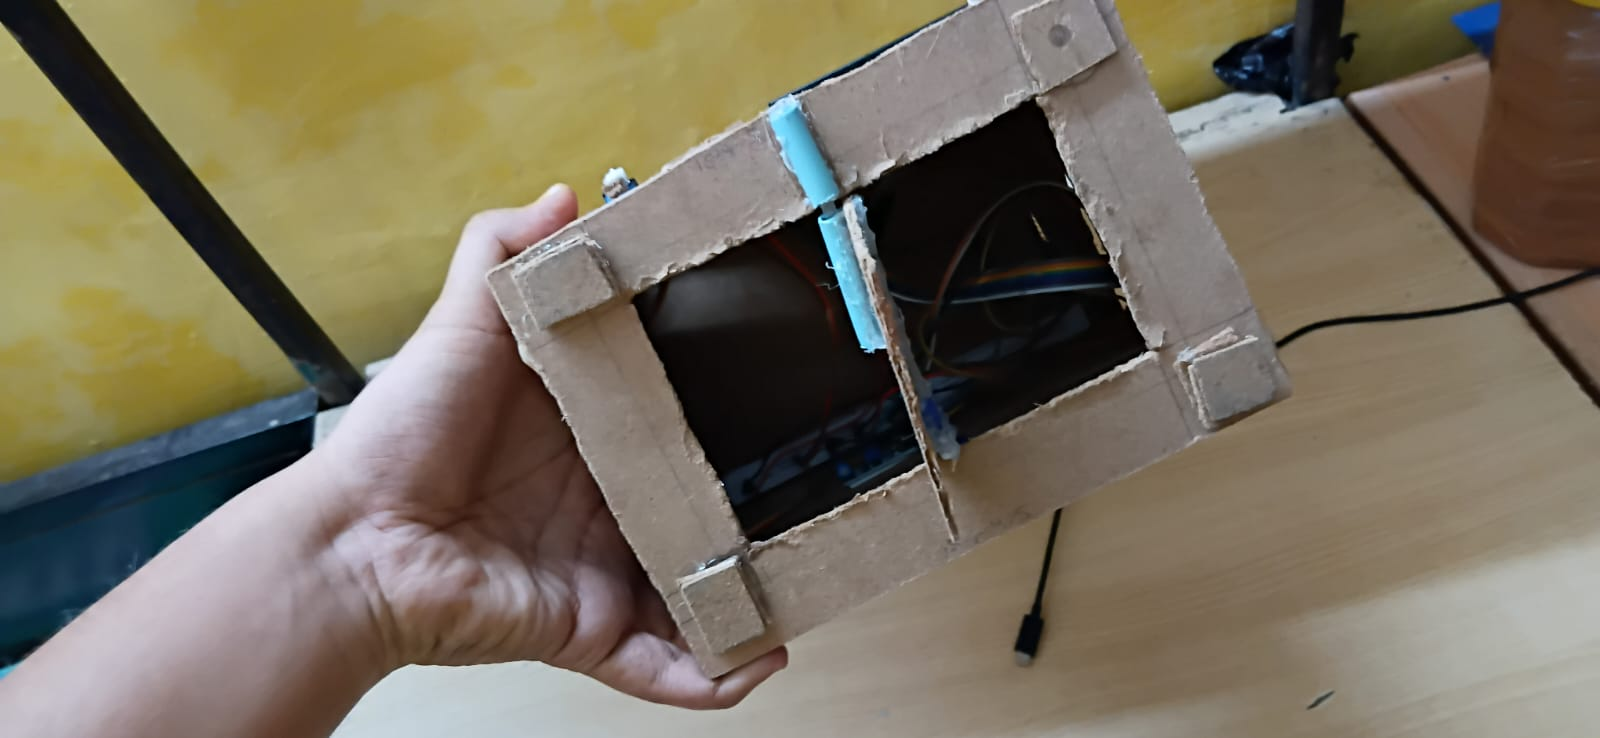
\includegraphics[width=0.45\textwidth]{atls-bottom.jpeg}
\caption{Hidden Safety Compartment Mechanism}
\end{figure}

\item The SW-420 vibration sensor continuously monitors physical tampering and forced break-in attempts.

\item If strong vibration or impact is detected:
\begin{itemize}
\item The alarm system is activated immediately.
\item Emergency security actions are executed.
\item Alert data is transmitted to Firebase.
\end{itemize}

\item The React web application provides:
\begin{itemize}
\item Real-time locker status monitoring
\item Remote password management
\item Intrusion alert visualization
\item Cloud-connected system monitoring
\item Live synchronization with ESP32
\end{itemize}

\end{enumerate}

\subsection{Technologies Used}

\begin{itemize}

\item \textbf{ESP32} --- Main microcontroller responsible for embedded processing and Wi-Fi communication.

\item \textbf{Arduino IDE} --- Development platform used for programming and uploading firmware to ESP32.

\item \textbf{Firebase Realtime Database} --- Cloud database used for real-time data synchronization and remote monitoring.

\item \textbf{React.js} --- Frontend framework used to develop the interactive web dashboard.

\item \textbf{HTTP Protocol} --- Communication protocol used for data transfer between ESP32 and cloud services.

\item \textbf{Embedded C/C++} --- Programming language used for hardware-level control and logic implementation.

\end{itemize}

\subsection{Web Dashboard}

The web-based dashboard provides a user-friendly interface for remote monitoring and control of the locker system. The dashboard displays locker status, intrusion alerts, authentication activity, and cloud-connected updates in real time. It also allows password management and remote system interaction through internet connectivity.

\begin{figure}[H]
\centering
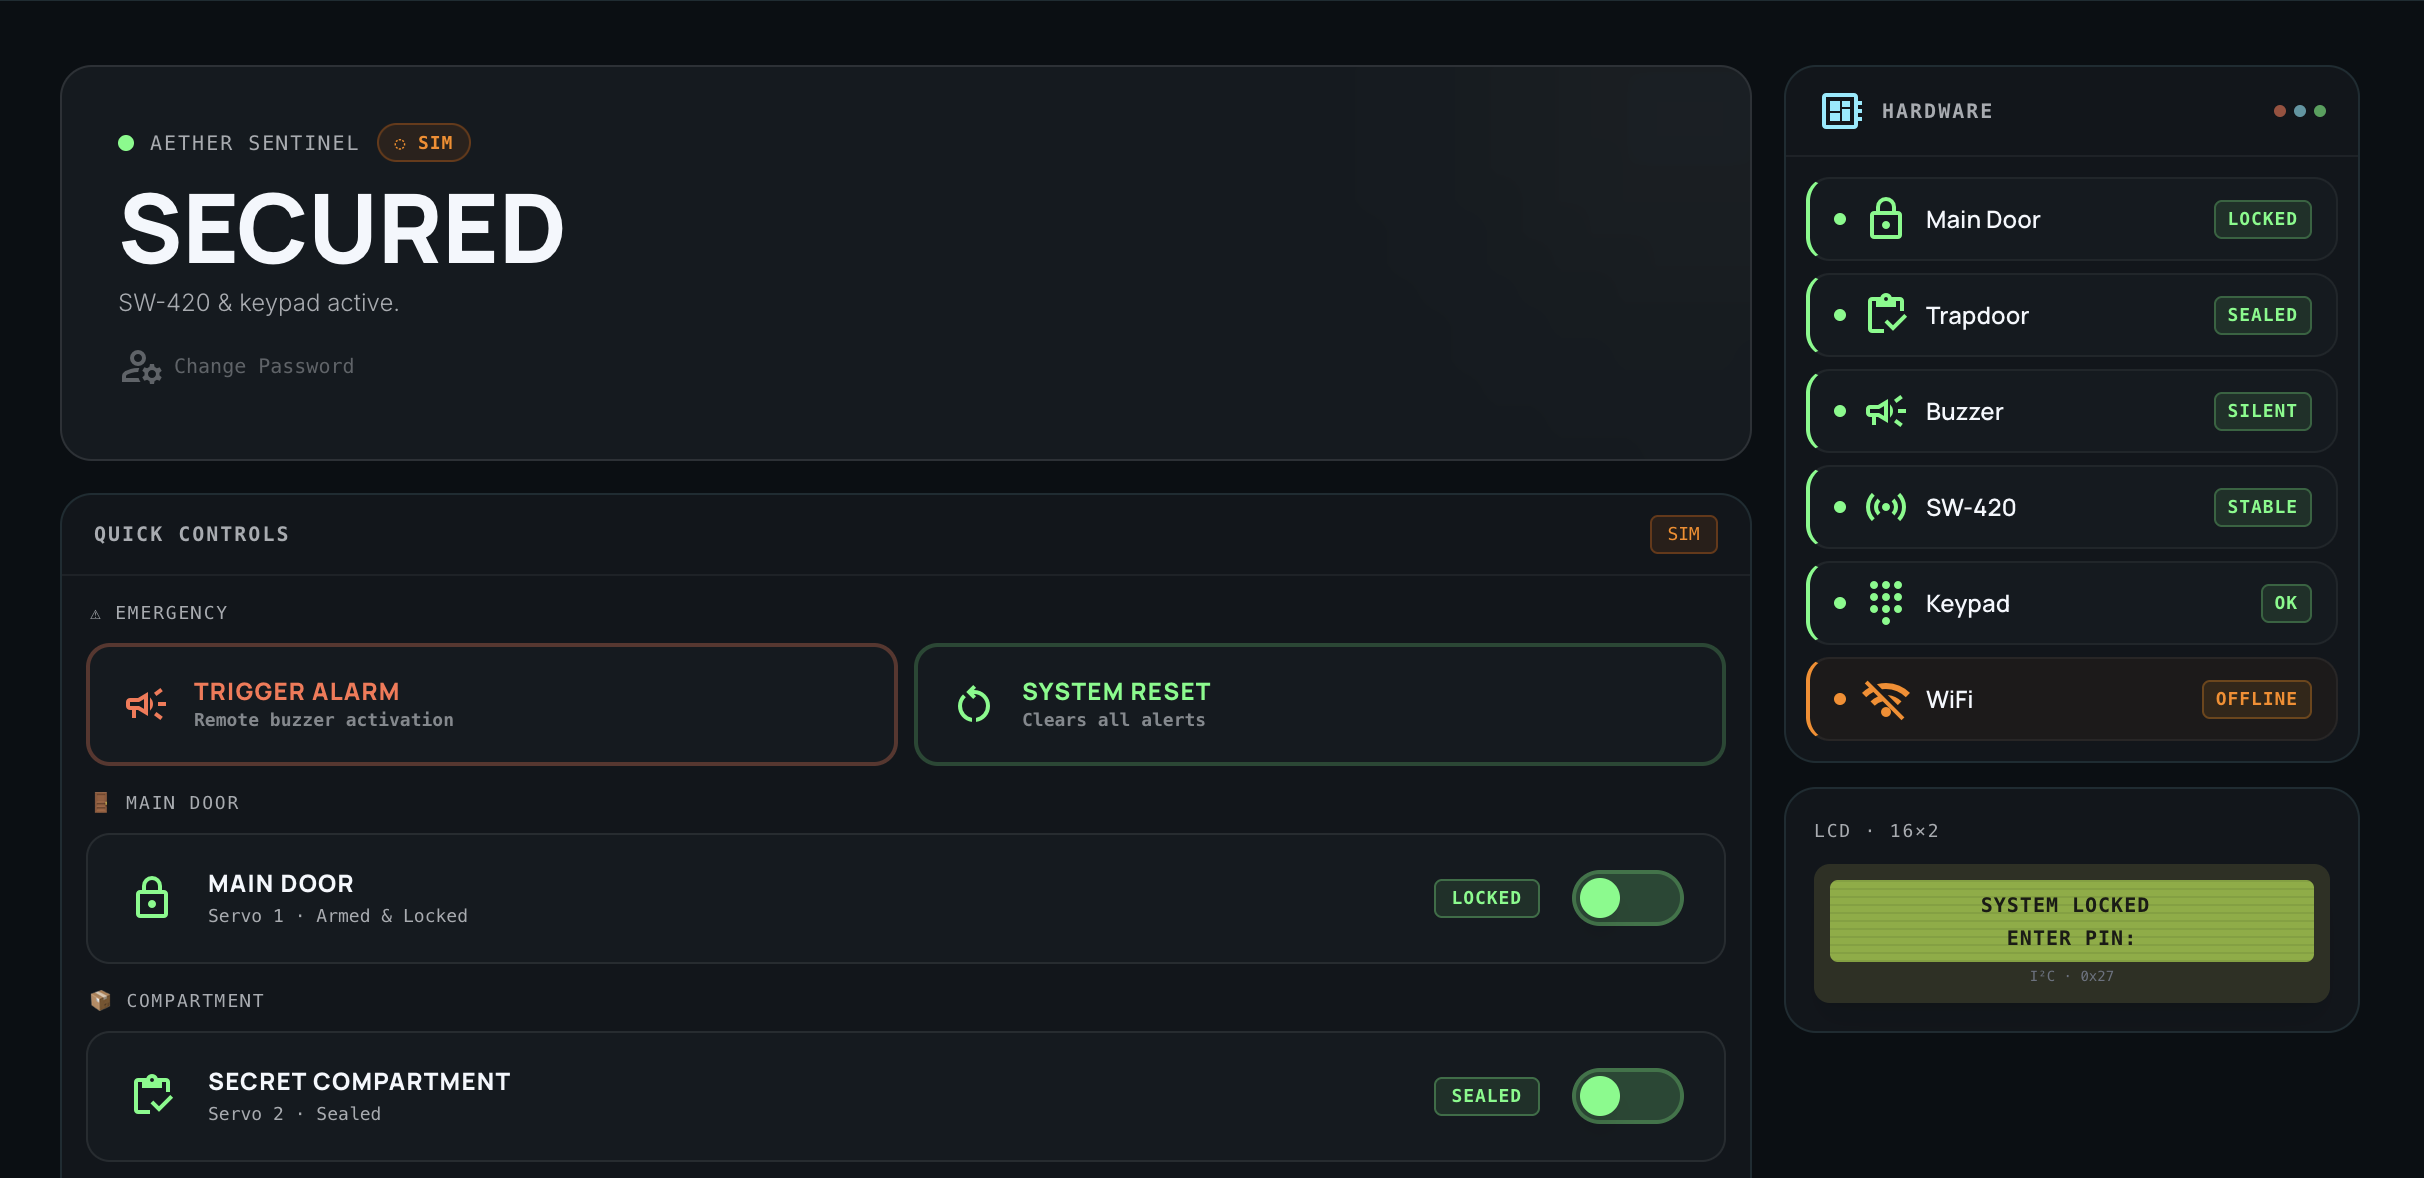
\includegraphics[width=0.45\textwidth]{website.png}
\caption{Web-Based Monitoring and Control Dashboard}
\end{figure}

% ================= X =================
\section{EXECUTION OF MODEL}

The developed prototype was tested under multiple operating conditions to verify system functionality and reliability.

\begin{itemize}
\item Correct password entry --- locker unlocks successfully
\item Incorrect password attempts --- alarm and intrusion alerts are triggered
\item Vibration/tampering detection --- hidden compartment activates and notifications are sent
\item IoT communication --- real-time updates synchronized with web dashboard
\end{itemize}

\begin{figure}[H]
\centering
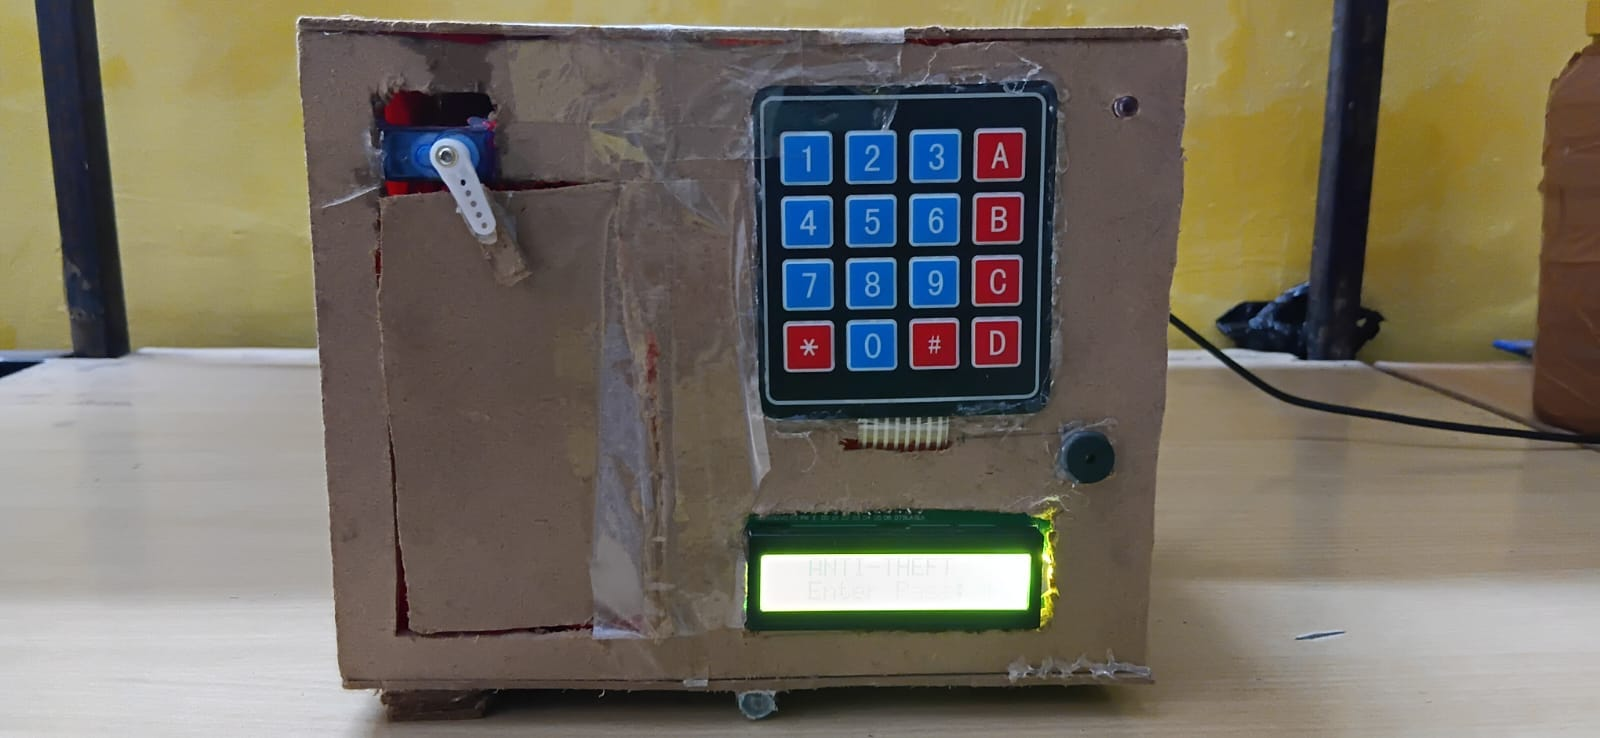
\includegraphics[width=0.45\textwidth]{atls-front.jpeg}
\caption{Front View of Developed Smart Locker Prototype}
\end{figure}
% ================= XI =================

\section{ADVANTAGES}

\begin{itemize}
    \item Improved security over normal lockers
    \item Real-time alerts to owner
    \item Password-based access control
    \item Intrusion detection using sensor
    \item Automatic locking mechanism
    \item Low cost and compact design
    \item Easy to install and maintain
    \item Suitable for IoT applications
\end{itemize}

% ================= XII =================
\section{APPLICATIONS}

\begin{itemize}

\item Home security lockers

\item Office and workplace storage systems

\item Bank locker security systems

\item Jewelry and valuables protection

\item Smart hostel and apartment lockers

\item IoT-based security applications

\item Document and file protection systems

\item Industrial equipment storage monitoring

\item Personal smart safety lockers

\item Educational institution storage systems

\end{itemize}


% ================= XIII =================

\section{FUTURE SCOPE}

\begin{itemize}

\item \textbf{Biometric Security} --- authentication using fingerprint and facial recognition:
Future improvements may include integrating AI-based face detection and fingerprint authentication systems to enhance security and automation. These features can provide multi-level user verification, allowing only authorized individuals to access the system. By combining computer vision, biometric authentication, and embedded technology, the project can become smarter, more reliable, and suitable for advanced real-world security applications.

\item \textbf{Mobile App Control} --- remote system management via smartphone:  
Enable users to control the locker, change password, and monitor status through a mobile application.

\item \textbf{Cloud Integration} --- online data storage and access:  
Use cloud platforms such as Firebase Realtime Database to store logs and manage system data.

\item \textbf{Advanced Sensors} --- high-precision motion detection:  
Integrate sensors like MPU6050 for improved and reliable tamper detection.

\item \textbf{Real-Time Alerts} --- instant notification system:  
Enhance alert mechanisms using internet-based communication for immediate user notification.

\item \textbf{Power Backup System} --- alternative energy source:  
Incorporate battery backup to ensure uninterrupted operation during power failures.

\item \textbf{Multi-Locker System} --- scalable locker management:  
Extend the system to manage multiple lockers in institutions such as banks or hostels.

\item \textbf{OTA Updates} --- over-the-air firmware updates:  
Allow remote software updates without requiring physical access to the system.


\end{itemize}

% ================= XIV =================
\section{CONCLUSION}

The Anti-Theft Smart Locker System with Secret Compartment and IoT Alerts successfully demonstrates a secure and intelligent approach to protecting valuables. The system integrates password-based authentication, vibration-based tamper detection, and an automated secret compartment mechanism to enhance security.

The implementation using a microcontroller (Arduino/ESP32) ensures efficient control of input, processing, and output components such as keypad, sensors, servo motor, and buzzer. The addition of IoT-based alerting enables real-time monitoring and notification, improving responsiveness to potential threats.

Overall, the project achieves its objective of providing a low-cost, reliable, and automated security solution. It also serves as a strong foundation for further enhancements such as biometric authentication, cloud-based control, and advanced intrusion detection systems.

% ================= REFERENCES =================
\section{References}

\begin{enumerate}

\item IoT Based Smart Security and Home Automation System, IEEE.\\
\url{https://ieeexplore.ieee.org/document/8457466}

\item Smart Door Lock System Using Arduino and IoT, IRJET.\\
\url{https://www.irjet.net/archives/V7/i5/IRJET-V7I5316.pdf}

\item Design and Implementation of Smart Locker Security System, IJERT.\\
\href{https://www.ijert.org/design-and-implementation-of-smart-locker-security-system}
{https://www.ijert.org/design-and-implementation-of-smart-locker-\\security-system}

\item Home Security System Using IoT and GSM, IEEE.\\
\url{https://ieeexplore.ieee.org/document/8688545}

\item Arduino Official Documentation.\\
\url{https://www.arduino.cc/en/Guide}

\item ESP32 Documentation by Espressif.\\
\url{https://docs.espressif.com/projects/esp-idf/en/latest/esp32/}

\item Firebase Realtime Database Documentation.\\
\url{https://firebase.google.com/docs/database}

\item React Official Documentation.\\
\url{https://react.dev/}

\item SW-420 Vibration Sensor Module.\\
\url{https://components101.com/modules/sw-420-vibration-sensor-module}

\item ESP32 Development Board.\\
\url{https://www.espressif.com/en/products/socs/esp32}

\item 16x2 LCD with I2C Module Guide.\\
\url{https://lastminuteengineers.com/i2c-lcd-arduino-tutorial/}

\end{enumerate}
\end{document}